\documentclass[11pt,a4paper]{article}

% Packages for formatting and graphics
\usepackage[utf8]{inputenc}
\usepackage{geometry}
\usepackage{graphicx}
\usepackage{listings}
\usepackage{xcolor}

% Page geometry
\geometry{margin=2.5cm}

% R code styling
\definecolor{codegreen}{rgb}{0,0.6,0}
\definecolor{codegray}{rgb}{0.5,0.5,0.5}
\definecolor{codepurple}{rgb}{0.58,0,0.82}
\definecolor{backcolour}{rgb}{0.95,0.95,0.92}

\lstdefinestyle{rstyle}{
    backgroundcolor=\color{backcolour},   
    commentstyle=\color{codegreen},
    keywordstyle=\color{magenta},
    numberstyle=\tiny\color{codegray},
    stringstyle=\color{codepurple},
    basicstyle=\ttfamily\footnotesize,
    breakatwhitespace=false,         
    breaklines=true,                 
    captionpos=b,                    
    keepspaces=true,                 
    numbers=none,                    
    showspaces=false,                
    showstringspaces=false,
    showtabs=false,                  
    tabsize=2,
    frame=single,
    rulecolor=\color{blue!30!black}
}

\lstset{style=rstyle}

\begin{document}

\begin{lstlisting}[language=R]
library(ggplot2)

# Set working directory to the script location
setwd("/home/alcafache/Documentos/PE/Exercicio1")

# Read the dataset with full path or ensure CSV is in correct directory
wine_data <- read.csv("winequality-white-q5.csv")

# Create the box plot with square root transformation of residual.sugar
plot <- ggplot(wine_data, aes(x = factor(quality), y = sqrt(residual.sugar))) +
  geom_boxplot(outlier.colour = "red", outlier.shape = 16, outlier.size = 2) +
  geom_jitter(width = 0.2, alpha = 0.3, size = 0.8) +
  labs(
    title = "Square Root of Residual Sugar by Wine Quality",
    x = "Wine Quality",
    y = "Square Root of Residual Sugar"
  ) +
  theme_minimal() +
  theme(
    plot.title = element_text(hjust = 0.5, size = 14),
    axis.title = element_text(size = 12),
    axis.text = element_text(size = 10)
  )
\end{lstlisting}

\vspace{1cm}

\begin{figure}[htbp]
    \centering
    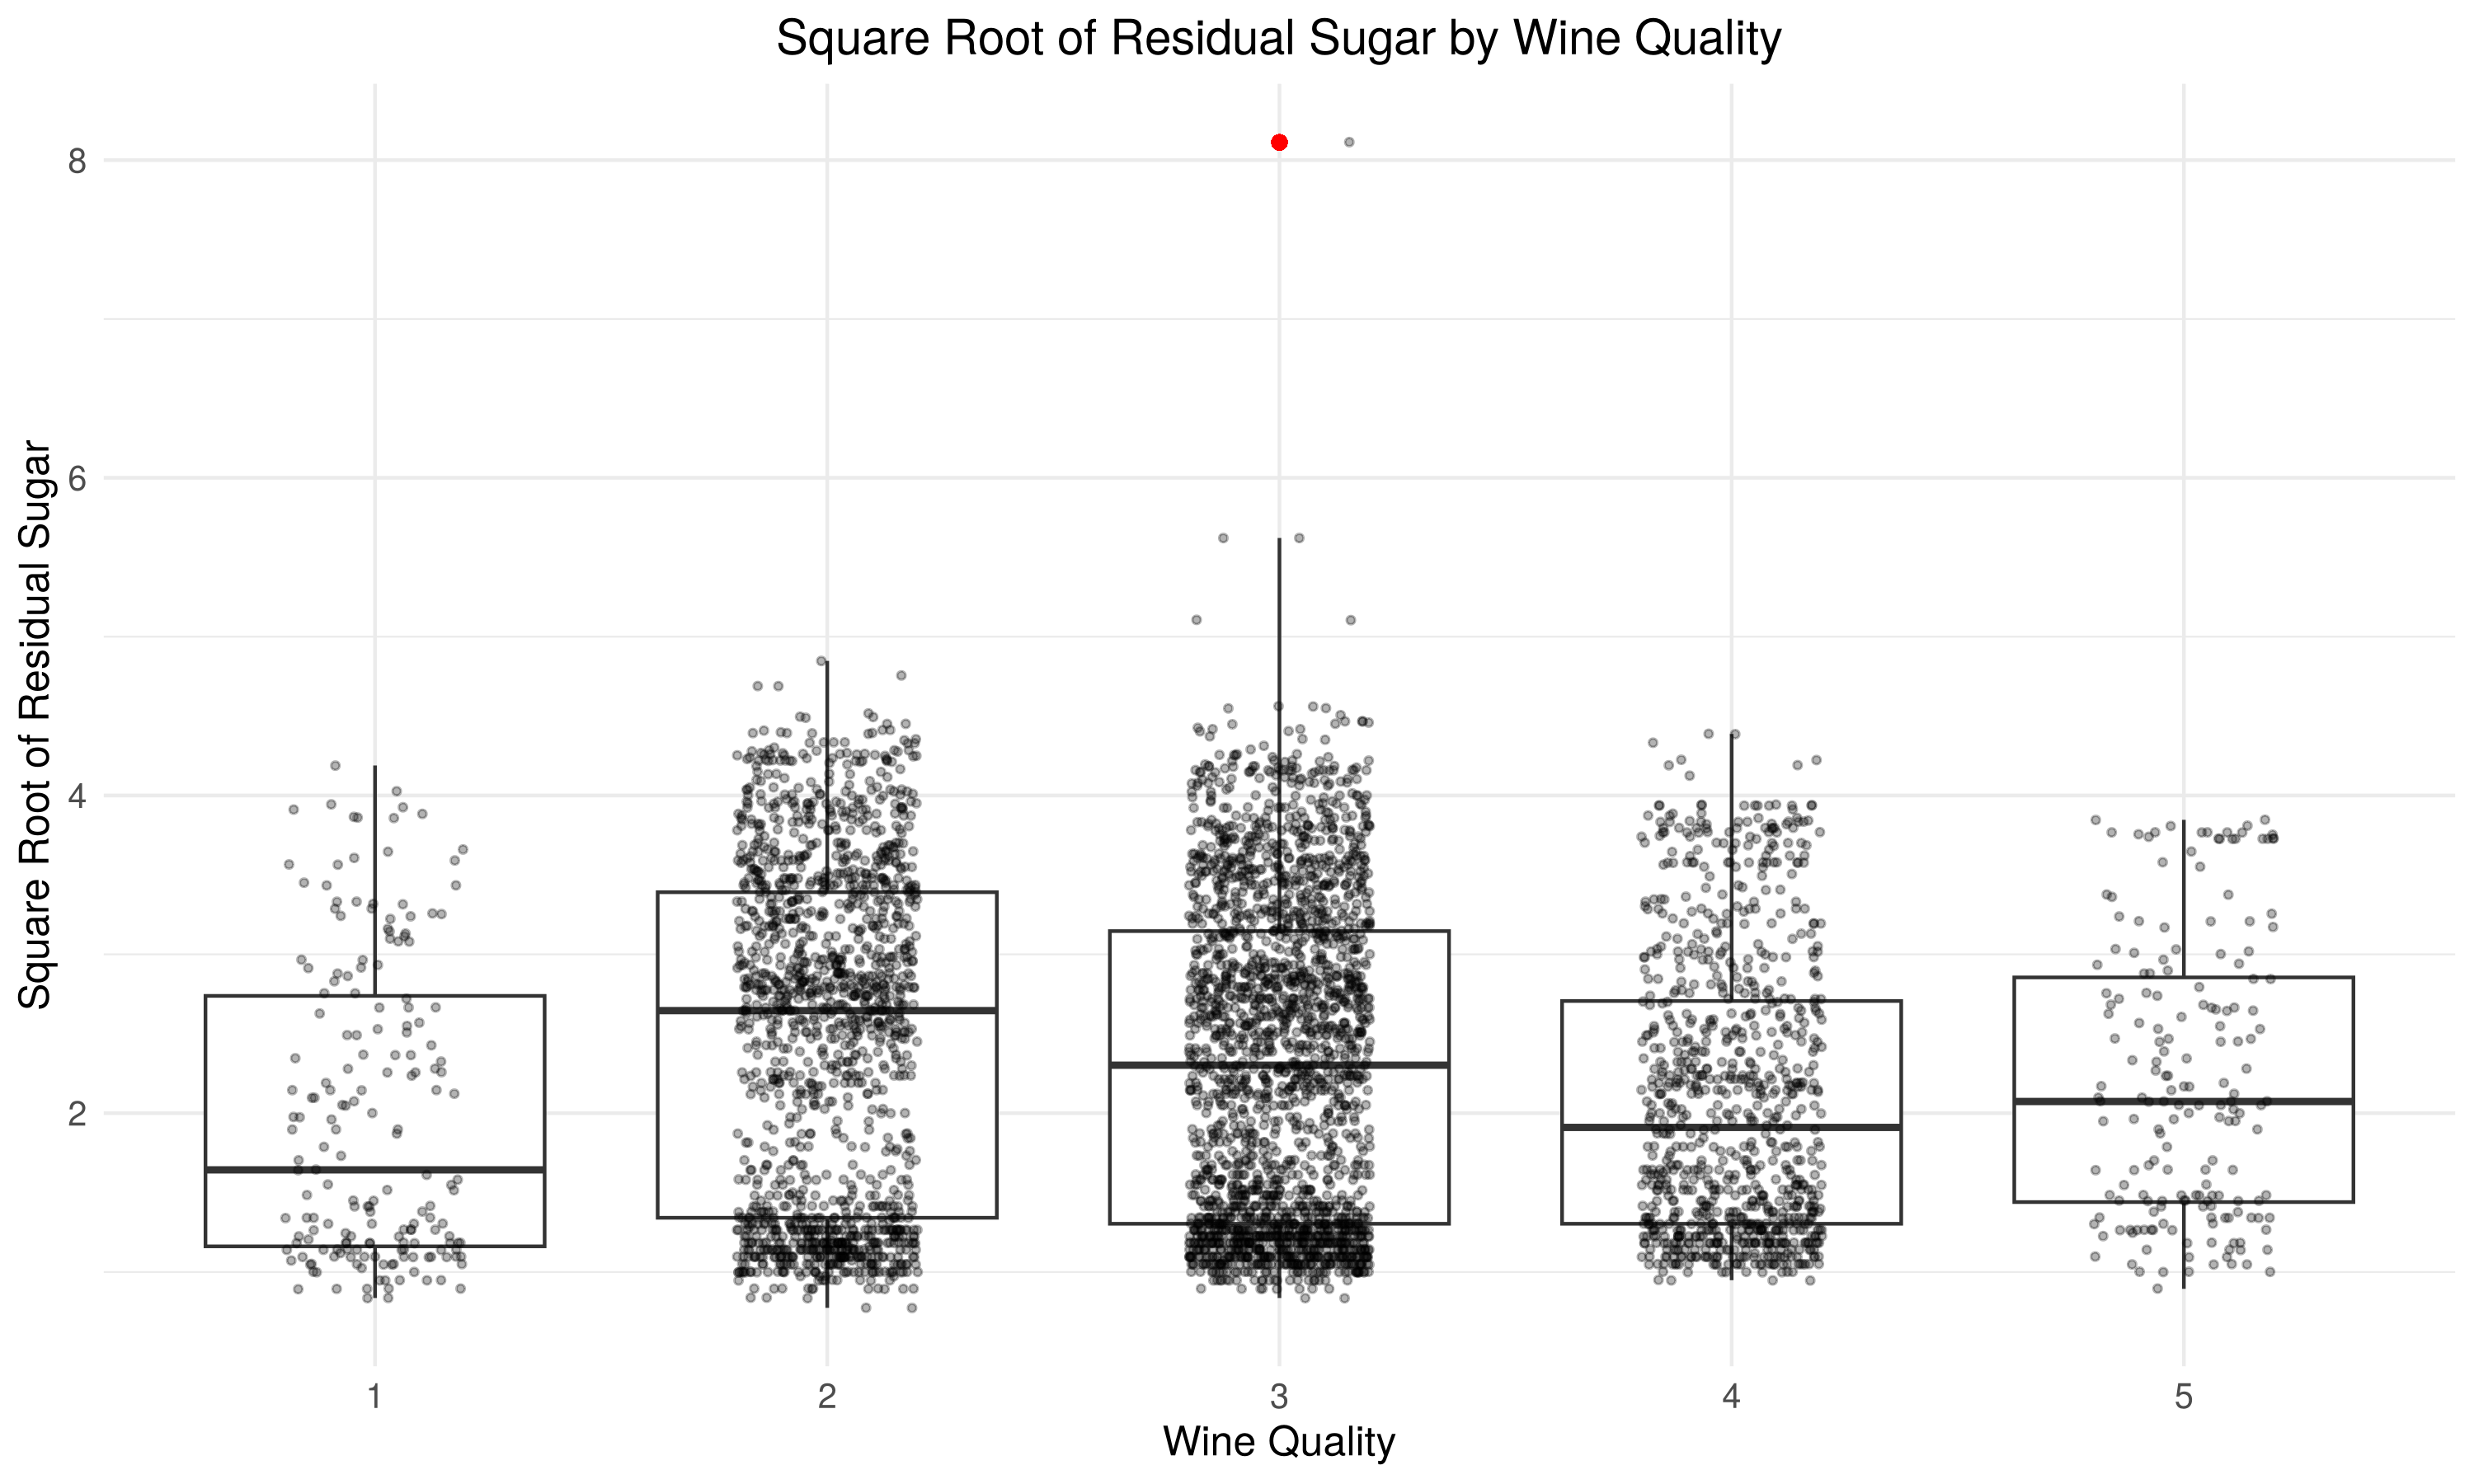
\includegraphics[width=0.9\textwidth]{wine_quality_boxplot.png}
\end{figure}

\end{document}
